\documentclass[11pt,a4paper]{article}
\usepackage[margin=2.2cm]{geometry}
\usepackage{graphicx,amsmath,amssymb,booktabs,xcolor,hyperref,float,caption}
\captionsetup{font=small,labelfont=bf}
\graphicspath{{figs/}}
\DeclareGraphicsExtensions{.pdf,.png}
\newcommand{\half}{\tfrac12}
\newcommand{\la}{\ell_a}
\newcommand{\kT}{k_BT}
\newcommand{\verdict}[2]{\textbf{\textcolor{#1}{[#2]}}}
\title{Crowded wall layers tilt less\\[2pt]\large What we measured, what we tested, and what is still open}
\author{Notes for B.~Loewe and T.~N.~Shendruk (prepared with Claude); updated 16 October, after all runs}
\date{16 October 2026}
\begin{document}
\maketitle

\begin{abstract}
The wall $+\half$ defects of an overcharged active cavity tilt from the wall normal. At leading order the tilt follows the flow-alignment law $\tau=\arccos(1/\lambda)$, $60^\circ$ at $\lambda=2$. With 10 seeds we find that this holds only for sparse wall layers. The tilt falls steadily as the wall defects crowd together, from $\approx64^\circ$ at spacings above 20 cells to $\approx42^\circ$ at 7 cells. The fall collapses on the wall-defect spacing. It appears in circles, ellipses and Cassini ovals, and it also appears in passive layers driven by an imposed vortex. We tested the candidate explanations in turn:
\begin{itemize}
\item measurement artefacts;
\item a weaker mean wall shear;
\item the defects' own active flow;
\item the finite-shear correction to the tilt law;
\item static elasticity, at a flat wall and in the circle;
\item the bulk spiral;
\item the continuum Q-tensor model in flat and circular geometries.
\end{itemize}
Most of these fail or explain only part of the drop. The picture that survives is a torque balance on the registry of the layer: the flow drives it towards the Leslie angle, an elastic pull drives it back towards the untilted registry, and the elastic pull per defect grows as the layer crowds. On this picture $\arccos(1/\lambda)$ is the flow-dominated limit, valid for sparse layers, and not a lower bound. Continuum models reproduce a crowding drop below $60^\circ$ only when their elastic pull points to the untilted registry, and the static tilt potential has the right crowding trend in its first harmonic. A quantitative prediction is still missing, because the second harmonic is not robust and the flow torque per defect is not known. The last sections list what the paper can safely claim and the open questions.
\end{abstract}

\section{Background and definitions}

\paragraph{Tilt law.} Relative to the wall normal, the anchored director turns by $(k-1)\phi$. A wall $+\half$ at azimuth $\phi_j$ therefore has its tilt locked to its position:
\begin{equation}
\tau_j=(2k-2)\phi_j+c .\label{eq:lock}
\end{equation}
A common tilt of the layer is a rigid shift of its registry. In shear next to a no-slip wall the far-field director settles at the Leslie angle $\theta_L$, with $\cos2\theta_L=1/\lambda$. The layer slides along this zero mode until the far field is aligned, so $\tau=2\theta_L=\arccos(1/\lambda)$. The master document adds a finite-shear correction from the torque passed through the band between wall and core:
\begin{equation}
\tau=\arccos\frac1\lambda+d\sqrt{\frac{\gamma_1 s}{K}}\,(\lambda^2-1)^{-1/4},\label{eq:corr}
\end{equation}
where $d$ is the core depth and $s$ the wall shear rate. The correction is always positive.

\paragraph{Definitions used throughout.}
\begin{itemize}
\item \textbf{Tilt.} $\tau=\psi-\theta_n$, the angle between the radial arm of the $+\half$ comet (the defect angle $\psi$ in \texttt{defects.dat}) and the outward wall normal. We checked analytically that the MPCD defect angle, the flat-wall direction of $\nabla\!\cdot\!Q$ and the ``head'' of the analytic calculations are all this same direction.
\item \textbf{Coherence.} $C=|\langle e^{i\tau_j}\rangle|$ over the wall defects of one frame (wall = within 4 cells of the wall).
\item \textbf{Tilt of the coherent layer.} The median over frames with $C>0.9$ of $|\arg\langle e^{i\tau_j}\rangle|$.
\item \textbf{Spacing.} $a=2\pi R/(2k-2)$ in circles, and the local site spacing $a(s)=\pi/(2\pi k/P-\kappa(s))$ in elongated cavities.
\item \textbf{Wall density.} $\rho=k/\pi R$.
\item \textbf{Alignment length.} $\ell_E=\sqrt{K/(\gamma_1 s\sqrt{\lambda^2-1})}$, the thickness of the shear boundary layer over which the director turns from the anchoring to $\theta_L$.
\end{itemize}

\section{The observation}

\begin{figure}[H]\centering
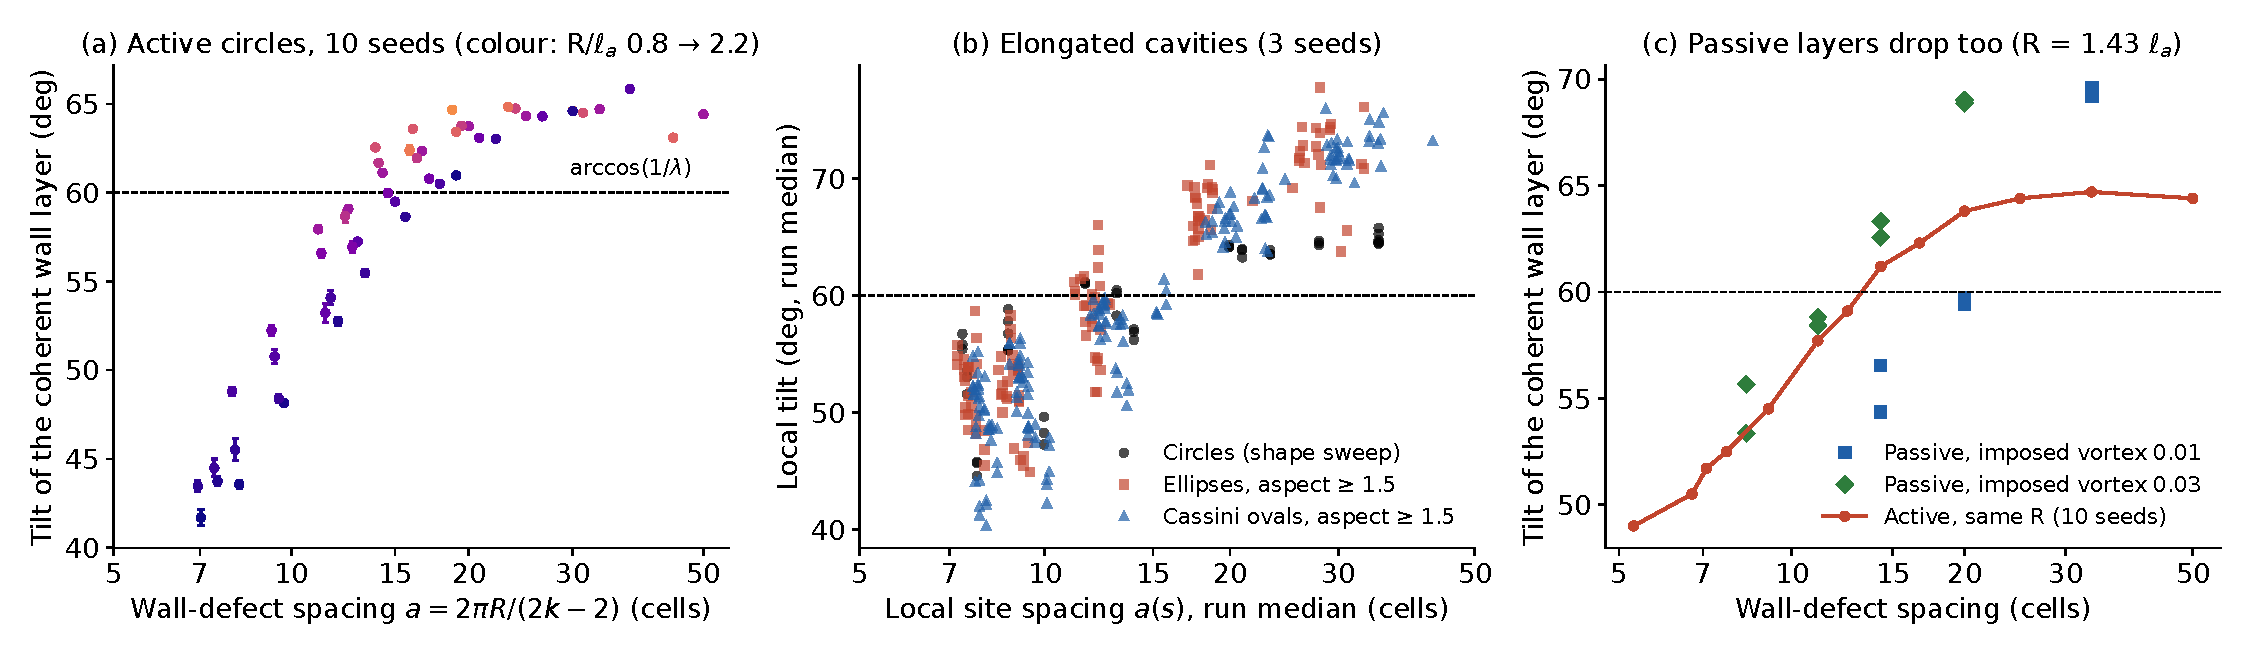
\includegraphics[width=\textwidth]{fig1_observation}
\caption{(a) Tilt of the coherent wall layer in active MPCD circles: $\lambda=2$, $\zeta=0.07$, $k=2$--10, $0.8\le R/\la\le2.2$, 10 seeds (mean $\pm$ s.e.\ per $(k,R)$). (b) Elongated cavities: local tilt of locally coherent triplets of wall defects against the local site spacing (run medians, 3 seeds). (c) Passive layers under an imposed vortex (two amplitudes) and active layers at the same radius $R=1.43\,\la$.}\label{fig:obs}
\end{figure}

\begin{itemize}
\item \textbf{The drop.} The tilt falls from $64.6^\circ$ ($\rho\approx0.04$) through 63.0, 59.2, 54.7 and 49.4 to $44.2^\circ$ ($\rho\approx0.14$). These are 506 runs with 10 seeds each (Fig.~\ref{fig:obs}a).
\item \textbf{Collapse on spacing.} A quadratic fit in $\log a$ leaves $1.7^\circ$ rms, against a raw spread of $7.0^\circ$. Fits in $k$ or $R$ alone leave $5$--$6^\circ$ (Fig.~\ref{fig:heat}). The tilt sits at $\approx64^\circ$ for $a\gtrsim20$ cells, crosses $60^\circ$ at $a\approx15$ and reaches $\approx42^\circ$ at $a=7$. A phenomenological form $\tau=\tau_L/(1+(a^*/a)^2)$ fits with $\tau_L=67.4^\circ$, $a^*=5.35$ cells and $2.0^\circ$ rms; it is a description, not a derivation.
\item \textbf{Elongated cavities} (Fig.~\ref{fig:obs}b). Measured from the local normal (the lock holds there too: resultant 0.94--0.98), ellipses and ovals show the same fall. Their sparse layers tilt more than circles, at $66$--$71^\circ$.
\item \textbf{Passive layers} (Fig.~\ref{fig:obs}c). Under an imposed vortex the tilt falls just as steeply, $69^\circ\to54^\circ$ between $a=20$ and $7.7$ at swirl 0.03. A stronger swirl raises the tilt at fixed spacing ($k=6$: $59.5^\circ$ at 0.01, $69^\circ$ at 0.03). Activity is therefore not required for the drop.
\end{itemize}

\begin{figure}[H]\centering
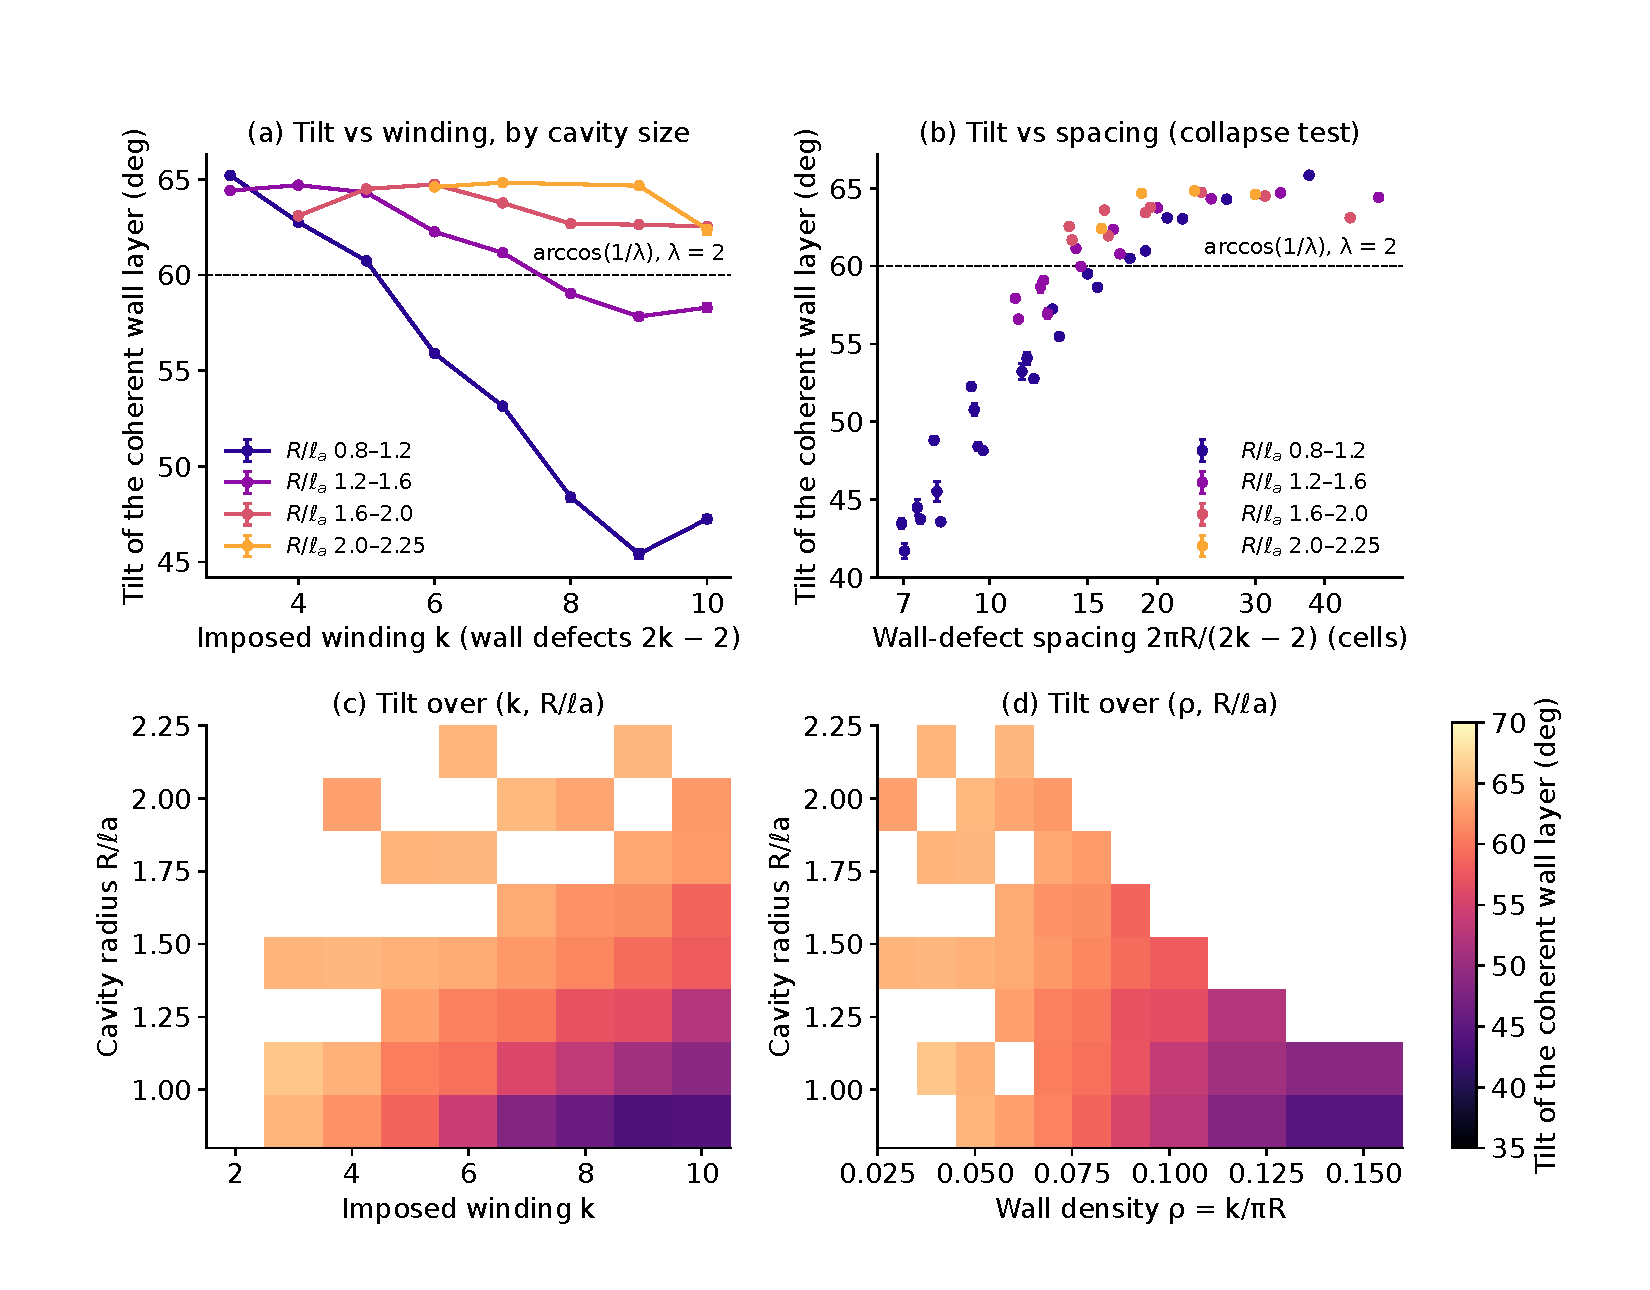
\includegraphics[width=0.85\textwidth]{fig_tilt_k}
\caption{Active circles (10 seeds). (a) Tilt against $k$ for four size bands. (b) Tilt against spacing: the collapse. (c, d) Tilt over $(k,R/\la)$ and over $(\rho,R/\la)$.}\label{fig:heat}
\end{figure}

\section{Test 1: is it a measurement effect? \verdict{red}{Mostly no}}

\begin{figure}[H]\centering
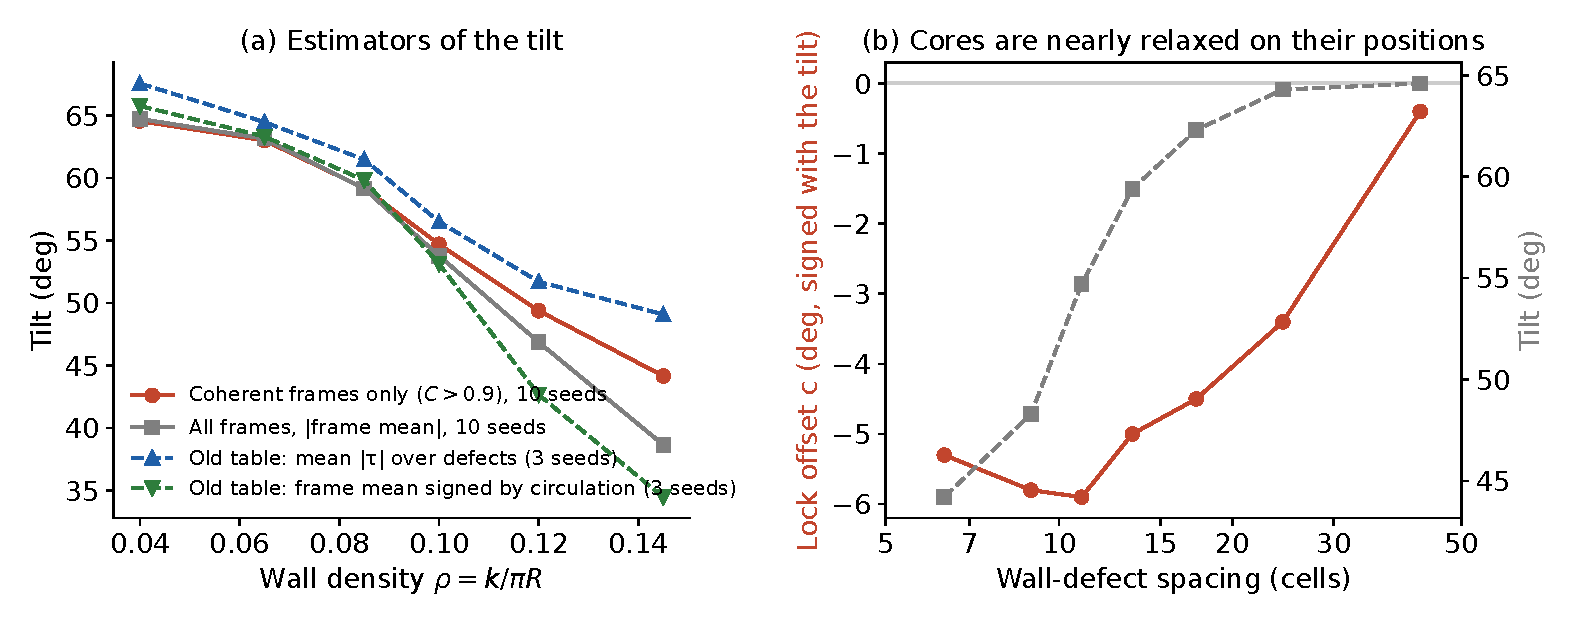
\includegraphics[width=0.85\textwidth]{fig2_measurement}
\caption{(a) Estimators of the tilt against wall density. The earlier table value signed by the circulation (3 seeds) overstates the drop at high $\rho$; the coherent-frame tilt does not. (b) Orientation offset $c$ of the cores from the lock, signed with the tilt, and the tilt itself, against spacing.}\label{fig:meas}
\end{figure}

\paragraph{Estimators.} The first report of the drop ($33$--$43^\circ$ at $\rho\ge0.12$) used the frame-mean tilt signed by the circulation and sampled every 100 t.u. Crowded layers scatter more and switch circulation more often, which pulls that average down. In addition, the column named \texttt{tilt\_coh} in that table is the magnitude of the mean angle, not the coherence. Restricting to frames in which the layer clearly shares one tilt ($C>0.9$) removes both effects. The drop survives, at a smaller size: $44^\circ$ instead of $38^\circ$ at $\rho\approx0.14$ (Fig.~\ref{fig:meas}a).

\paragraph{Are the cores relaxed?} Your point was that the logarithmic interaction assumes each defect's orientation has relaxed to its minimum. Unrelaxed orientations exert torques. We measured the offset $c$ of each frame's cores from the lock, Eq.~\eqref{eq:lock}. Sparse layers are relaxed ($c=-0.4^\circ$). Crowded layers are twisted back toward the normal by $5$--$6^\circ$, and the resultant falls from 0.99 to 0.97 (Fig.~\ref{fig:meas}b). This is real, but it accounts for only $\approx5^\circ$ of the $\approx20^\circ$ drop. The rest is the registry: crowded defects sit closer to their homeotropic sites.

\paragraph{Is the angle measured the same way everywhere? Yes.} All analyses measure the angle between the radial arm of the comet and the outward normal:
\begin{itemize}
\item MPCD uses the tracker angle (Vromans--Giomi, the direction of $\nabla\!\cdot\!Q$);
\item the continuum codes use $\nabla\!\cdot\!Q$ directly;
\item the analytic calculations use $2\theta_{\rm rest}$, which is the same direction.
\end{itemize}
On seeded rings with known geometry the tracker recovers the intended 0, 60 and 120$^\circ$ to within 1--2$^\circ$ in median for spacings $\ge11$ cells. On about 5000 coherent director frames at $R=31.8$, the tracker tilt and the tilt from $\nabla\!\cdot\!Q$ of the MPCD director field agree at every $k$, with a median difference $\le0.8^\circ$. Both show the drop ($64.5\to48^\circ$). Tracker positions show no offset against seeded positions.

\section{Test 2: is it the flow? \verdict{orange}{Partly}}

\begin{figure}[H]\centering
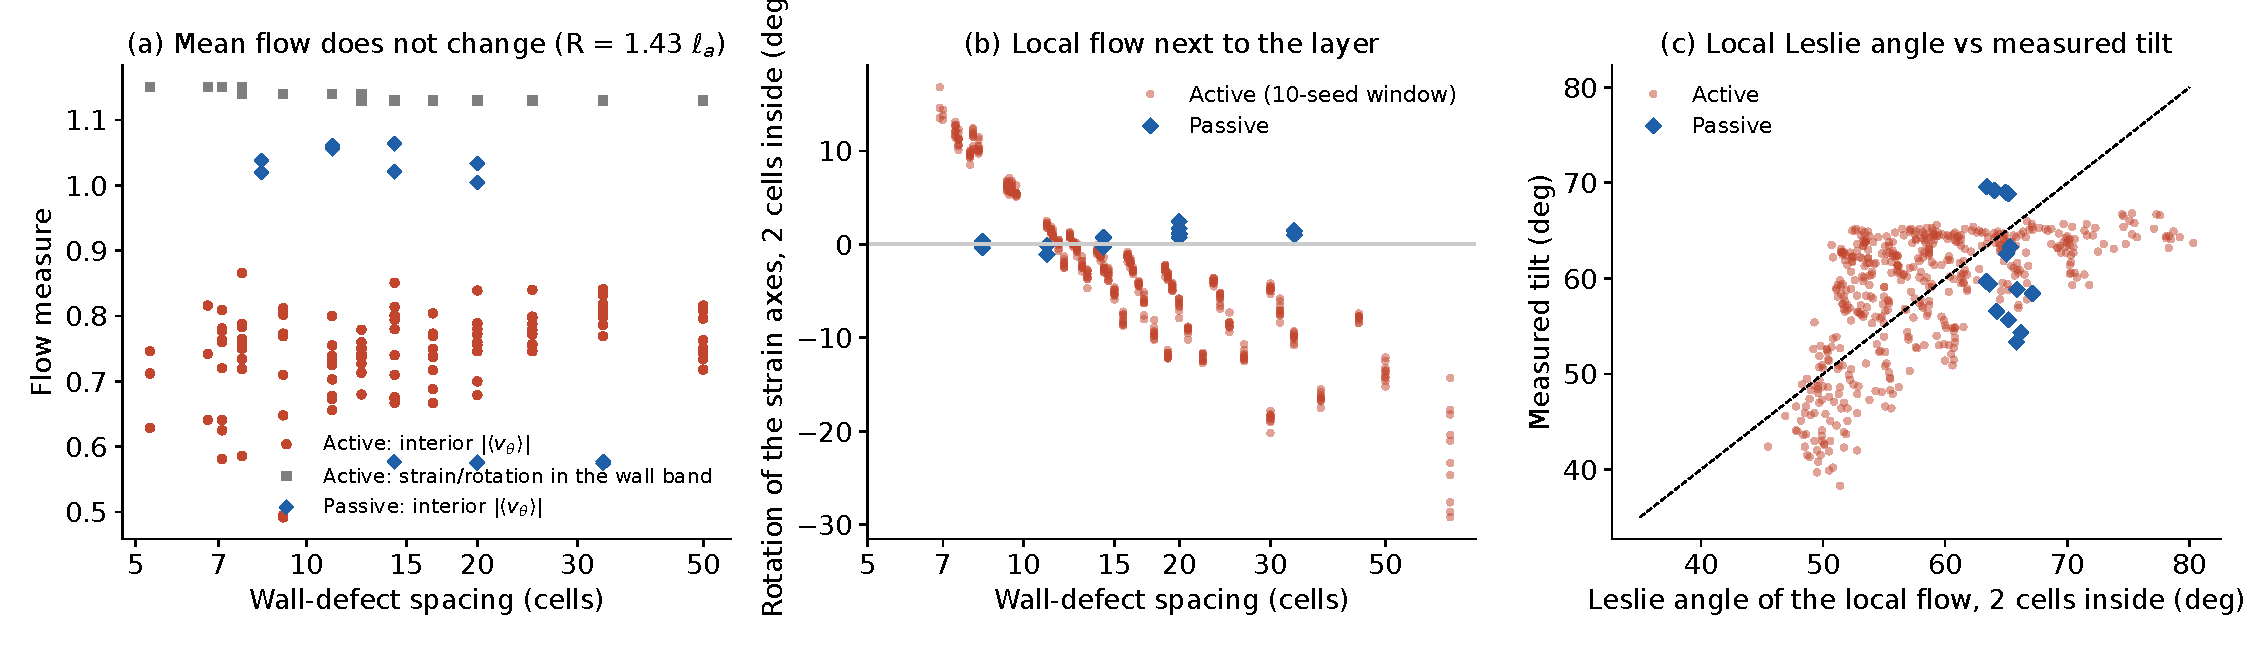
\includegraphics[width=\textwidth]{fig3_flow}
\caption{(a) Interior circulation and strain/rotation ratio in the wall band at fixed $R=1.43\,\la$: neither changes with spacing. (b) Rotation of the principal strain axes two cells inside the layer, in each wall defect's own frame: active layers (10-seed window) and passive layers. (c) Leslie angle of that local flow against the measured tilt.}\label{fig:flow}
\end{figure}

\paragraph{Mean wall shear: \verdict{red}{fails}.} Your first idea was that the layer's self-flow opposes the circulation, so a denser layer weakens the wall shear. At fixed $R$, however, the azimuthally averaged wall-band shear is the same for every $k$ (strain $\approx0.09$--$0.10$, strain/rotation 1.10--1.15), and so is the interior circulation. The tilt law also predicts no dependence on the shear magnitude, only on the strain/rotation ratio, and that ratio is unchanged.

\paragraph{Local flow at the layer: \verdict{orange}{works for active, fails for passive}.} The defects' flow lobes repeat with period $a$ and cancel in the azimuthal mean, so we sampled the flow in each wall defect's frame.
\begin{itemize}
\item \textbf{Active layers.} Two cells inside the layer the strain axes rotate steadily, from $-17^\circ$ (sparse) through 0 at $a\approx13$ to $+11^\circ$ (crowded). The Leslie angle of that local flow tracks the measured tilt bin by bin: $49.6/52.0/57.0/65.1^\circ$ against $45.8/51.2/60.8/64.4^\circ$ for $a$ = 5--8/8--12/12--20/20--60 (Fig.~\ref{fig:flow}b,c).
\item \textbf{Passive layers.} The local flow is plain wall shear at every spacing: strain-axis rotation $0\pm1^\circ$, local Leslie angle $63$--$67^\circ$. The tilt still falls.
\item \textbf{The active core.} It carries the defect's own extensional self-flow: $e_{xx}\approx-0.02$, strain axes rotated by $-21$ to $-27^\circ$ at the core. Along the wall this flow runs against the circulation in sparse layers.
\end{itemize}
\emph{Reading:} the local-flow change in active layers is the active self-flow and goes with the tilt. It is not needed for the drop, because passive layers fall equally with an unchanged local flow. In active layers it is most likely a consequence of the crowded, less tilted layer rather than its cause.

\section{Test 3: elasticity and pinning \verdict{orange}{Right ingredient, not quantitative}}

\paragraph{What was already established (master \S28--29c; RESEARCH.md 6--8 Oct).}
\begin{enumerate}
\item \textbf{The lock.} $\tau_j=(2k-2)\phi_j+c$ holds with resultant length 0.99.
\item \textbf{The elastic minimum is the untilted layer.} Tails sit on the homeotropic sites. To first order in $K_1-K_3$ the potential is exactly $\propto\cos\tau$, and the bulk $+1$ adds a further $\cos\tau$ term because it prefers the bend vortex.
\item \textbf{The active registry is pinned, but not at that minimum.} From any initial director the active layer ends at $\pm63$--$64^\circ$, one sign per circulation sense, with no creep. It sits away from the energy minimum and is held there by the activity. It behaves as a stick--slip system under an imposed swirl.
\item \textbf{The passive registry is not pinned.} It is frozen spontaneous symmetry breaking and only creeps; under imposed flow it slides.
\item \textbf{The torque balance.} Beyond first order, $E(\tau)=A_1\cos\tau+A_2\cos2\tau+\dots$. With a drive $D\sin\tau$ the stable tilt is $\cos\tau^*=-(D+A_1)/(4A_2)$, which requires $A_2>0$. At $k=6$ the computed $A_2\approx5\,\kT$ gives $\approx35^\circ$; the measured $63^\circ$ needs $A_2\approx15$--20.
\end{enumerate}
In this framework $\arccos(1/\lambda)$ is not a lower bound. It is the limit in which the flow dominates the pinning. A layer whose pinning pulls it towards the untilted registry tilts less, and can tilt below $60^\circ$, when the pinning becomes comparable to the flow torque.

\paragraph{The sign of the pinning decides (continuum, Fig.~\ref{fig:cont}).} The Landau--de Gennes flat wall with MPCD's $K_1/K_3=1.82$ relaxes to $\tau=180^\circ$ (radial arm into the bulk). Under shear it tilts \emph{more} at small spacing (69--89$^\circ$). The exact first-order flat-wall calculation agrees: $E=A\cos\tau$ per defect, with $A>0$ (preferring $180^\circ$) for crowded or deep layers and $A<0$ for sparse or shallow ones (Fig.~\ref{fig:el}a). A model whose pull points to $\tau=0$ ($K_1/K_3=0.55$) reproduces the drop: on the flat wall $64.6\to51.5^\circ$ (spacing $30\to8$), and in the circular disk $63.6\to54.7^\circ$ (spacing $31\to4.8$). Melting the wall order adds little. We checked $K_1$ and $K_3$ three times (MPCD fluctuation fits with the mean director verified along $x$; continuum modulation tests; analytic formula). MPCD has $K_1\approx42>K_3\approx23\,\kT$, so the $0.55$ model has the wrong anisotropy for MPCD. It is a stand-in for ``pull towards $\tau=0$'', not a model of MPCD. In the circle the pull towards $\tau=0$ comes from the bulk vortex term, which is absent at a flat wall.

\paragraph{The tilt potential across crowding (Fig.~\ref{fig:pot}a,b).} We relaxed the full anisotropic Frank energy (rigid cores; R 31.8; $k=3$--20) for several bulk models.
\begin{itemize}
\item \textbf{Bulk $+1$ as a point at the centre:} $A_1<0$ at every spacing, per defect roughly constant for $k\ge6$.
\item \textbf{Bulk split into two $+\half$, or a disordered interior} (three $+\half$ and one $-\half$ at random, closer to MPCD, whose interior has order $\le0.2$): $A_1$ changes sign with crowding. Sparse layers are pushed towards $180^\circ$ and crowded layers pulled towards $0^\circ$, with the crossover at a spacing of $\approx10$--20 cells. This is robust to grid and core size.
\item \textbf{The second harmonic $A_2$} is small, falls with crowding, and changes with grid and core. A torque balance with a drive calibrated at $k=6$ (per defect or per wall length) gives erratic, non-monotonic predictions. It does \emph{not} reproduce the smooth $64\to49^\circ$ decline.
\end{itemize}
The resting-state test (passive MPCD, seeded rings at $\tau_0=0/60/120^\circ$, no flow) keeps every seeded registry for 100--300\,t.u. Afterwards the bulk pair returns to the wall and coherence is lost. The slow drifts go up for sparse layers and down for the most crowded one (single seeds; weak evidence, consistent with the sign change of $A_1$).

\paragraph{Static stiffness.} At first order in a point-bulk circle, both the registry stiffness and the core-twist stiffness per defect \emph{soften} with crowding (Fig.~\ref{fig:el}b). This was the basis for the earlier (wrong) statement that elasticity is excluded. That statement used a model whose pull does not change sign; the split and disordered bulk models above do change sign.

\begin{figure}[H]\centering
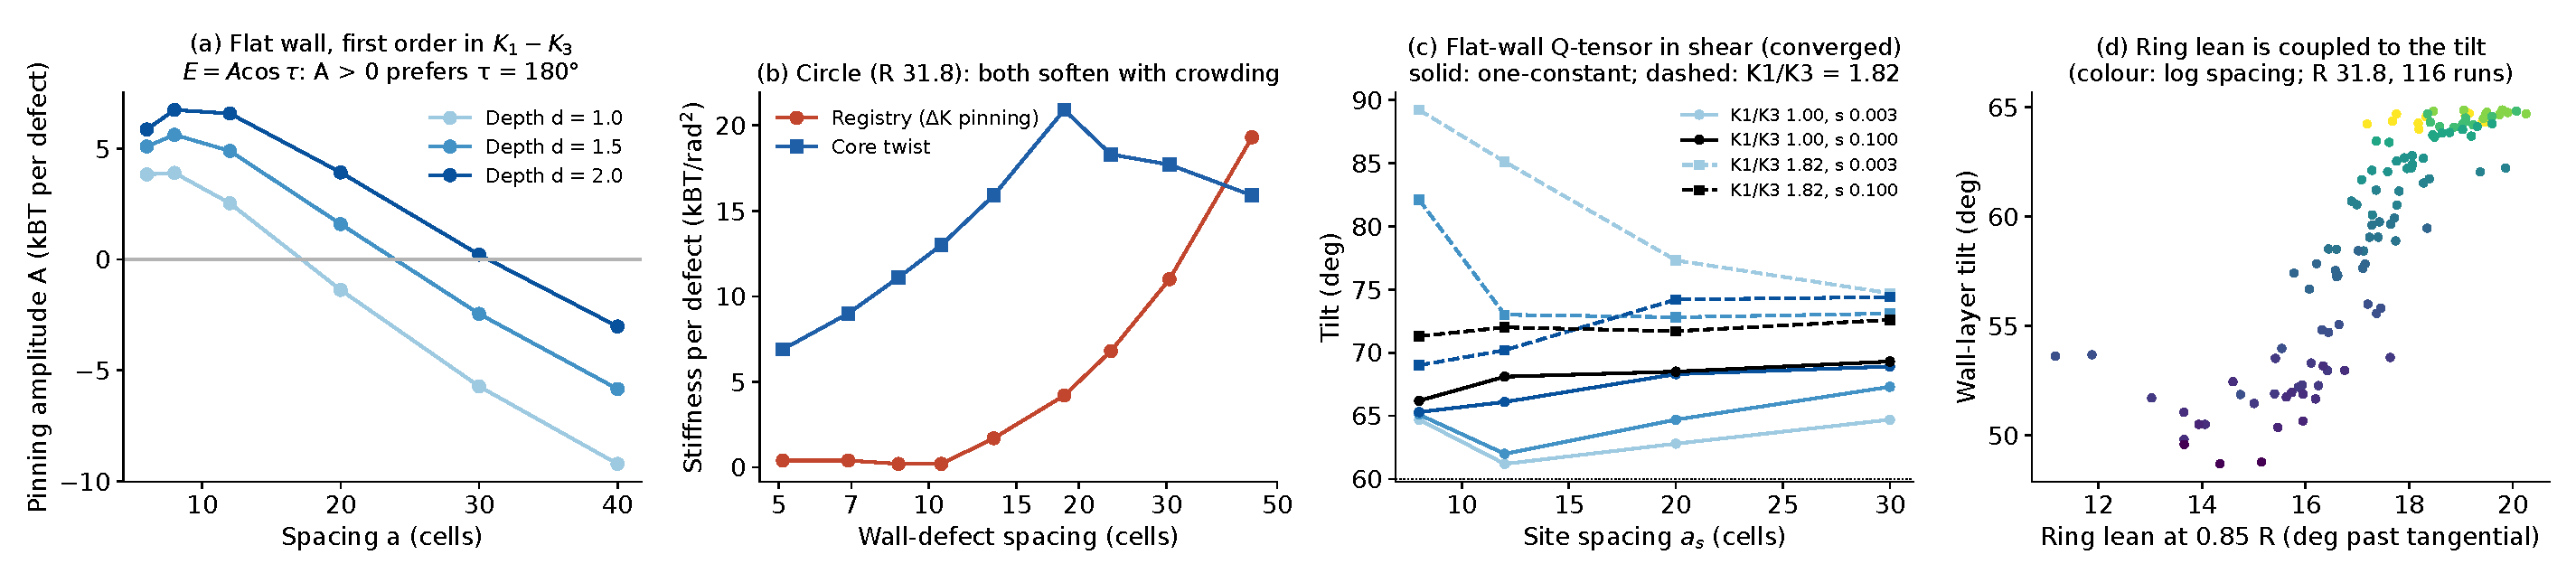
\includegraphics[width=\textwidth]{fig4_elastic}
\caption{(a) Flat-wall registry pinning at first order in $K_1-K_3$: $E(\tau)=A\cos\tau$ per defect, with $A>0$ preferring $\tau=180^\circ$. (b) Circle with a point bulk $+1$, first order: registry and core-twist stiffness per defect. (c) Flat-wall Landau--de Gennes model in shear. (d) Lean of the ordered director ring at $0.85R$ against the wall tilt.}\label{fig:el}
\end{figure}

\begin{figure}[H]\centering
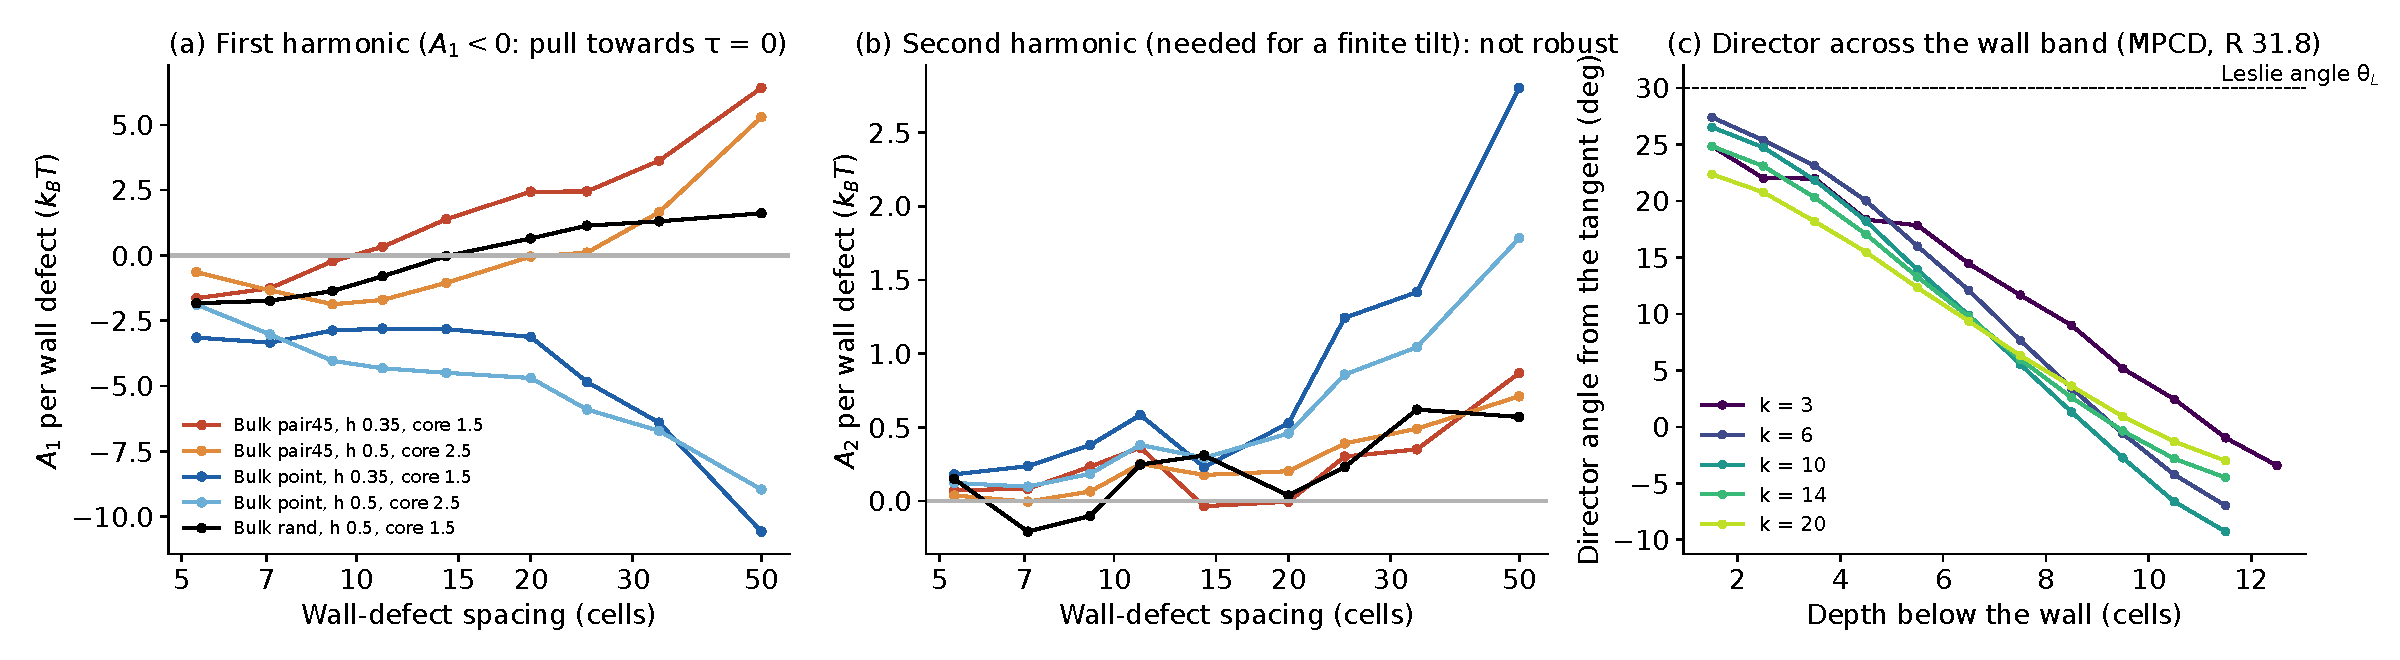
\includegraphics[width=\textwidth]{fig7_potential_band}
\caption{(a, b) Harmonics of the tilt potential per wall defect against spacing (R 31.8), for point, split (pair at $\pm0.45R$) and disordered (random) bulk models and two numerical resolutions. (c) MPCD director angle from the local tangent against depth, for several $k$ at $R=31.8$.}\label{fig:pot}
\end{figure}

\section{Test 4: depth and the alignment length \verdict{orange}{Orders the data, mechanism open}}

\begin{figure}[H]\centering
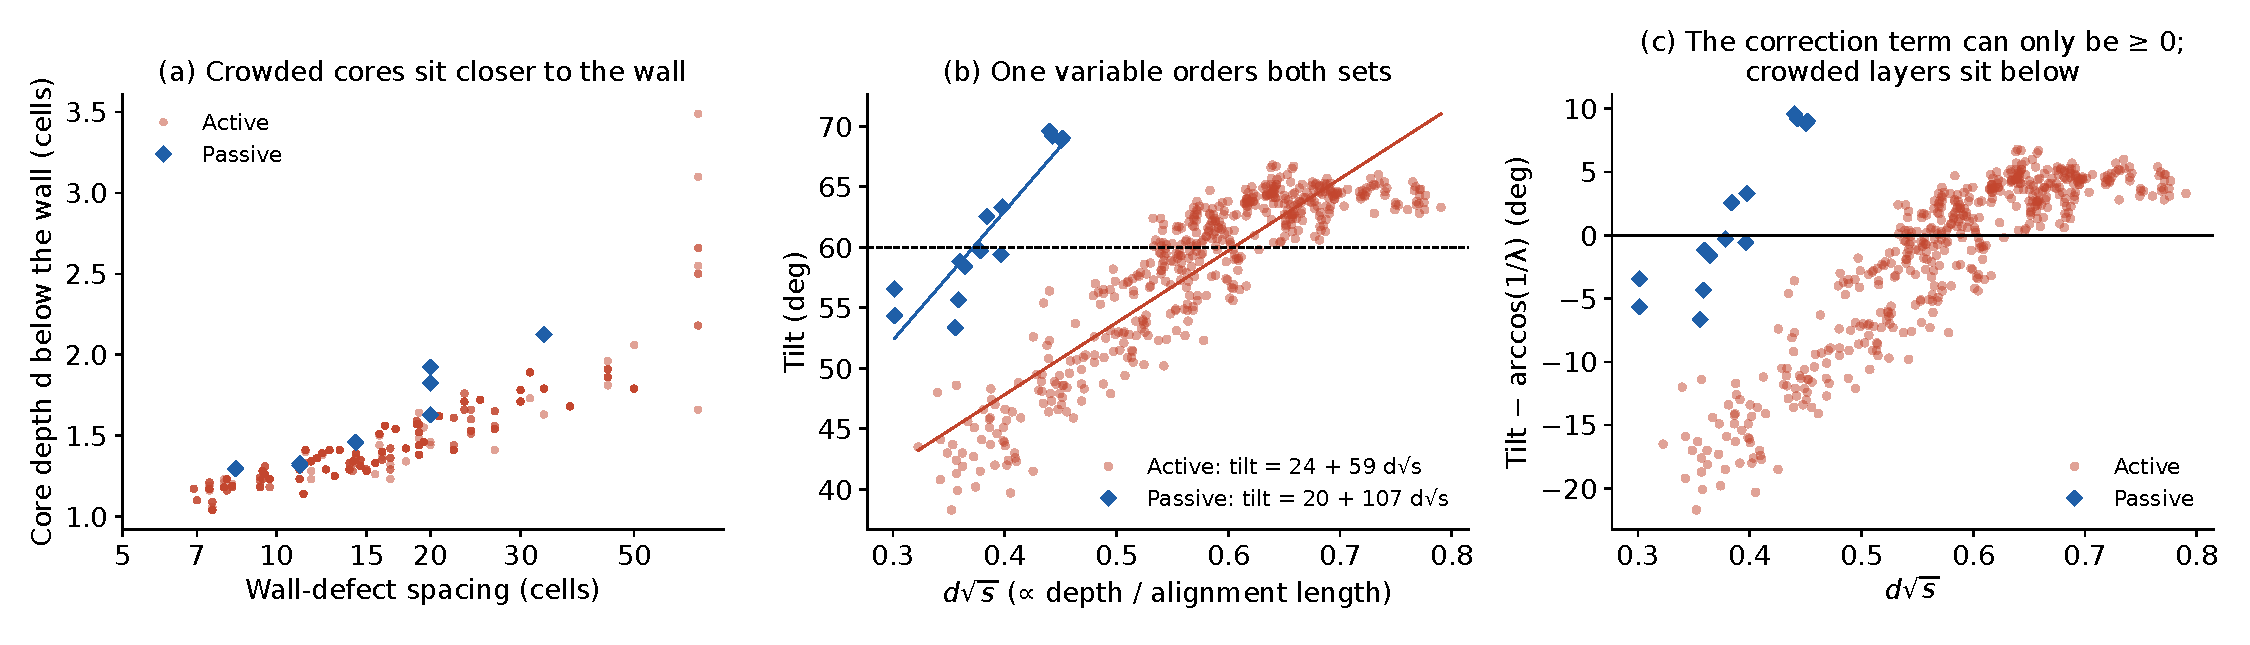
\includegraphics[width=\textwidth]{fig5_depth}
\caption{(a) Core depth below the wall against spacing, active and passive. (b) Tilt against $d\sqrt{s}$ with linear fits. (c) Tilt minus $\arccos(1/\lambda)$: the correction term of Eq.~\eqref{eq:corr} can only be positive.}\label{fig:depth}
\end{figure}

\paragraph{What fits.} Crowded cores sit closer to the wall: median depth $1.7\to1.2$ cells (active) and $1.9\to1.3$ (passive) between sparse and crowded layers. The tilt is linear in $d\sqrt{s}$ for both sets:
\begin{itemize}
\item passive: $\tau\approx20^\circ+107\,d\sqrt{s}$, with $2.3^\circ$ rms (raw $5.6^\circ$);
\item active: $\tau\approx24^\circ+59\,d\sqrt{s}$, with $3.0^\circ$ rms (raw $6.7^\circ$).
\end{itemize}
Both fits beat spacing alone ($3.4^\circ$/$3.5^\circ$) and depth alone ($4.2^\circ$/$4.3^\circ$). The shear rate matters at fixed depth: passive $k=8$ at $d=1.46$ gives $55.5^\circ$ at $s=0.043$ and $63^\circ$ at $s=0.072$. Since $d\sqrt{s}\propto d/\ell_E$, the variable that orders the data is the core depth measured in units of the shear boundary layer.

\paragraph{Independent test: shear at fixed spacing (new, 19 Oct).} Passive circles under an imposed vortex at fixed $k$ (6: spacing $\approx19$; 13: $\approx7.8$), with the
forcing varied tenfold. The line fitted above on the crowding runs predicts these runs without refitting (Table~\ref{tab:shearscan}): at $k=6$ the tilt rises from
$54.6^\circ$ to $66.9^\circ$ as $d\sqrt{s}$ grows, with residuals $-0.4$ to $+2.1^\circ$; at $k=13$ the cores sit shallower ($d\approx1.3$ against 1.7--2.0), so at the
same wall shear ($s\approx0.063$) the tilt is $12$--$15^\circ$ lower, again on the line (residuals $-3.1$, $-0.8^\circ$). Spacing and shear act only through $d\sqrt{s}$ in this range.
The line overshoots at the strongest forcing ($k=6$: $68.5^\circ$ against $73^\circ$; $k=13$, $A=0.1$: $63^\circ$ against $73^\circ$, few coherent frames), where the tilt saturates.
\begin{table}[H]\centering\small
\begin{tabular}{lcccccc}\toprule
run & $k$ & depth $d$ & wall shear $s$ & $d\sqrt{s}$ & tilt & predicted \\\midrule
$A=0.005$ & 6 & 1.99 & 0.026 & 0.32 & 54.6 & 54.8\\
$A=0.01$ & 6 & 1.82 & 0.043 & 0.38 & 60.4 & 60.8\\
$A=0.02$ & 6 & 1.66 & 0.063 & 0.42 & 66.9 & 64.8\\
$A=0.05$ & 6 & 1.99 & 0.062 & 0.50 & 68.5 & 73.1\\
$A=0.02$ & 13 & 1.29 & 0.064 & 0.33 & 52.0 & 55.1\\
$A=0.05$ & 13 & 1.33 & 0.062 & 0.33 & 54.9 & 55.7\\
$A=0.1$ & 13 & 1.29 & 0.147 & 0.50 & 62.8 & 73.2\\\bottomrule
\end{tabular}
\caption{Shear scan at fixed spacing (runs/swirl\_shear), predicted by $\tau=20.3^\circ+106.7\,d\sqrt{s}$ fitted on the passive crowding runs. $k=6$, $A=0.1$ and $k=13$, $A\leq0.01$
have no coherent layer ($k=13$ ejects only for $A\geq0.02$, and only partly at $A=0.02$: bulk $+0.5$, 10\% coherent frames). Source: master/theory/tiltcrowd/shear\_scan\_dsqrts.txt.}\label{tab:shearscan}
\end{table}

\paragraph{The drop shrinks with flow alignment (new, 19 Oct).} Active circles of the same size (area 2500) with a sparse ($k=6$, spacing $\approx17$) and a
crowded ($k=14$, spacing $\approx6.8$) layer, $\lambda=2$--6. Coherent-layer tilts, sparse/crowded: $62.5/47.6^\circ$ ($\lambda=2$), $71.9/65.7^\circ$ (3),
$74.9/71.2^\circ$ (4), $78.0/77.4^\circ$ (6). The crowding drop falls from $15^\circ$ to $6$, $4$ and $<1^\circ$. Both layers keep their full $2k-2$ and bulk $+1$ at every $\lambda$.
Stronger alignment overrides whatever pins the crowded layer, as a flow-versus-pinning balance with a drive growing with $\lambda$ would predict; this is
a constraint for any quantitative model (source: master/theory/robust/robust\_sets.txt).

\paragraph{Why the correction term itself fails.} Eq.~\eqref{eq:corr} has the right trend on the sparse side: as $d$ shrinks the positive excess shrinks, which explains a fall from 64--69$^\circ$ toward $60^\circ$. But the term is positive by construction, so it cannot produce tilts below $60^\circ$, and crowded layers sit at 44--55$^\circ$ (Fig.~\ref{fig:depth}c). Fitted with its leading term fixed at $60^\circ$, it leaves residuals that still correlate with spacing ($+0.8$). The fitted intercepts of 20--24$^\circ$ say that, in the data, the tilt is not ``$60^\circ$ plus a correction'' at all.

\paragraph{The director across the band (Fig.~\ref{fig:pot}c).} In MPCD the director angle from the tangent peaks right inside the layer, at 25--28$^\circ$ (sparse) and 22--25$^\circ$ (crowded). It never reaches $\theta_L=30^\circ$, and it decays to zero by 9--10 cells, where the wall-sign shear ends. The layer tilt exceeds twice that peak by $15^\circ$ (k\,3), $9^\circ$ (k\,6), $5^\circ$ (k\,10) and $3$--$4^\circ$ (k\,14--20). So two things fall together with crowding: the defects' over-rotation past the local field (which behaves like the positive finite-depth correction), and the local director itself. That twice the peak angle is 45--55$^\circ$ for every $k$ suggests that the sparse-layer agreement with $\arccos(1/\lambda)$ is partly a compensation: incomplete alignment in a thin shear zone, plus over-rotation of deep cores.

\paragraph{A hypothesis that would explain the sign.} The layer's periodic distortion extends only $\sim a/2\pi$ from the wall, and the alignment length in MPCD is $\ell_E\approx1.4$--$2.7$ cells. For sparse layers ($a/2\pi\approx3$--8) the distortion reaches past $\ell_E$, and the layer locks to a fully aligned far field. For crowded layers ($a/2\pi\approx1$--1.6) it lies inside the boundary layer, so the layer would lock to a field that has only partly rotated toward $\theta_L$. This would give $\tau<60^\circ$. It needs something that resists the zero-mode sliding, because the one-constant continuum shows no drop even when $a/2\pi\ll\ell_E$.

\paragraph{Continuum test of this regime: \verdict{red}{inconclusive}.} In the flat-wall Q-tensor model $d/\ell_E$ stays at 0.05--0.29, while MPCD has 0.5--1.2. At strong shear ($s=0.3$) the continuum defect is pushed onto the first grid row, and at $s=1$ it is absorbed into the wall. The continuum cannot reach the MPCD regime, where the cores stay 1.2--2 cells deep.

\section{Test 5: continuum models \verdict{orange}{No drop without the right pinning}}

\begin{figure}[H]\centering
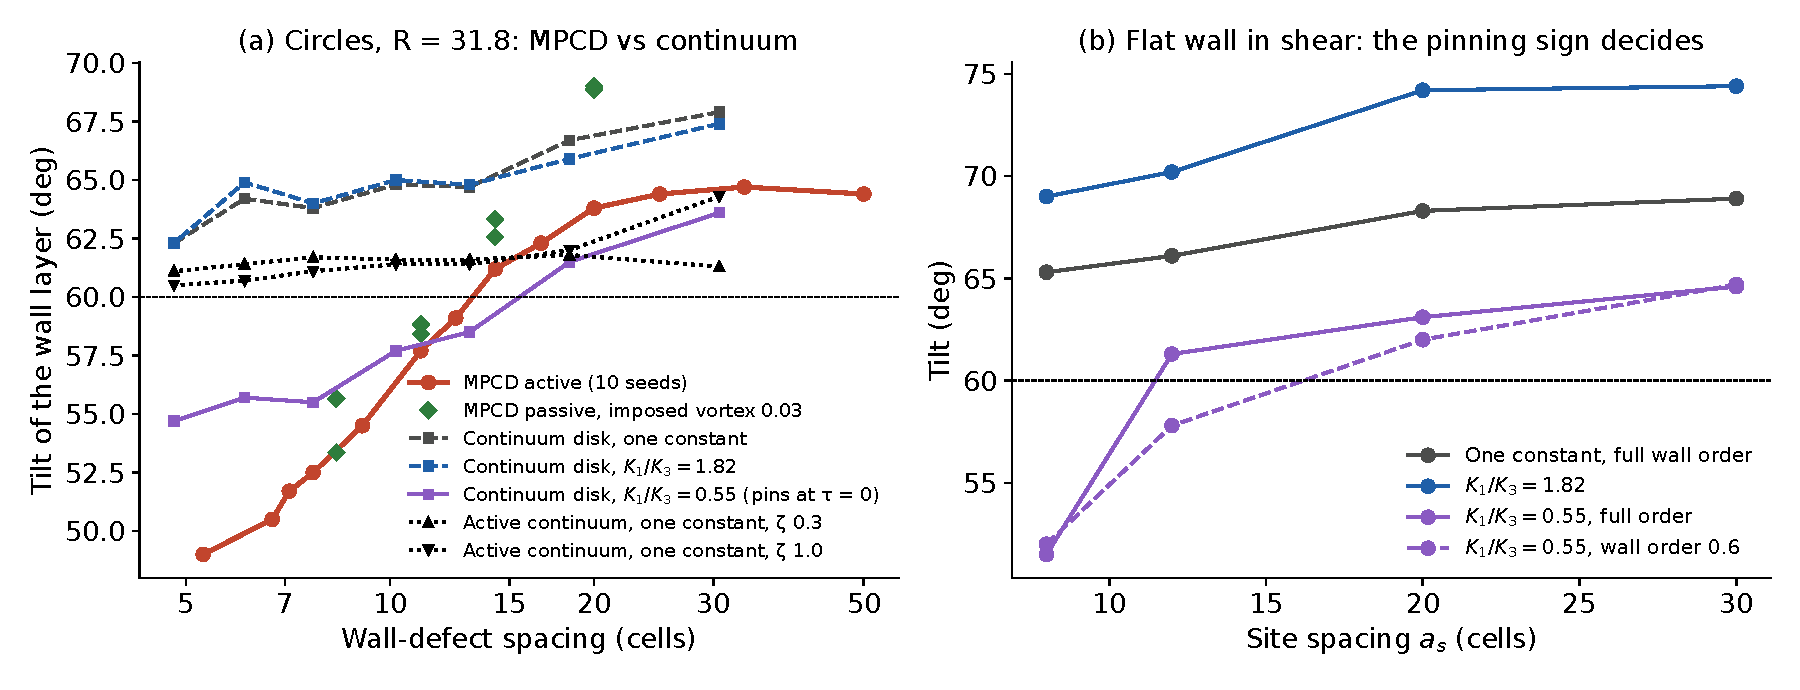
\includegraphics[width=\textwidth]{fig6_continuum}
\caption{(a) Circles at $R=31.8$: MPCD (active, 10 seeds; passive under an imposed vortex) against continuum disks (passive with an imposed no-slip vortex, $U=1$, three elastic models; active with backflow, one constant). (b) Flat wall in shear ($s=0.03$): one constant, $K_1/K_3=1.82$ and $0.55$, and a melted wall.}\label{fig:cont}
\end{figure}

\begin{itemize}
\item \textbf{Passive disk, one constant or $K_1/K_3=1.82$:} mild fall from $\approx68^\circ$ to $62^\circ$ toward $\arccos(1/\lambda)$, never below it.
\item \textbf{Passive disk, $K_1/K_3=0.55$:} $63.6\to54.7^\circ$, below $60^\circ$ at spacing $\lesssim15$. This is a smaller drop than MPCD's.
\item \textbf{Active disk} (one constant, backflow, $\zeta=0.3$ and 1): the self-organised overcharged state appears at every $k$, and the tilt stays at 60.5--64$^\circ$. There is no crowding drop.
\item \textbf{Flat wall with finite anchoring} (Rapini--Papoular): with the layer kept ($W=1$) the tilt is 65--71$^\circ$; for weaker anchoring the defect is absorbed into the wall. MPCD's anchoring is in fact strong: the wall-cell director deviates by only 2.4--5$^\circ$ between defects at every spacing. What drops with crowding is the order at the wall ($0.91\to0.79$; $0.65$ at cores).
\item \textbf{Active disk with noise or stronger activity} (new, 19 Oct; one constant, backflow, $k=4$ and 16). Additive noise on $Q$ ($D=0.002$, 0.01) leaves the tilt
at $61.4$--$61.5^\circ$ for both $k$: noise alone gives no drop. At $\zeta=3$ the tilt is $65.2^\circ$ ($k=4$) against $57.3^\circ$ ($k=16$): an $8^\circ$ crowding drop
appears with activity. The $\zeta=3$ disk stays laminar (coherence 1.00, steady tilt, two bulk $+\half$, no pairs) with a fully ordered bulk spiral (order 1.1), so this drop needs neither turbulence nor the loss of the spiral; noise disorders the spiral (order 0.7) without a drop. Its cores sit at $d/\ell_E=1.28$ ($k=4$) and 0.42 ($k=16$), bracketing the MPCD range (0.5--1.2); the crowded value is limited by resolution (core depth 0.39 cells, grid 0.5).
\item \textbf{Activity scan, $\zeta=3$--10} (new, 20 Oct). Both disks keep a single vortex up to $\zeta=8$; the crowding drop is $7.9^\circ$ ($\zeta=3$), 7.7 and $8.1^\circ$ ($\zeta=4$, 5), then 9.4, 10.2 and $10.7^\circ$ ($\zeta=6$--8). A few bulk $-\half$ appear from $\zeta=4$; sustained pair creation starts at $\zeta=7$ (sparse) and 8 (crowded); at $\zeta=8$ the sparse disk's spiral breaks up (order 0.19), the crowded one stays ordered (1.17); at $\zeta=10$ the crowded disk loses its vortex. $d/\ell_E$ stays at 1.2--1.7 (sparse) and 0.42--0.53 (crowded, resolution-limited). The scan cannot separate turbulence from the growing wall shear: the largest step comes before sustained pair creation. The continuum drop is about half of the MPCD drop at the same radius ($14^\circ$) at $\zeta=3$--5 and about three-quarters at $\zeta=8$.
\item \textbf{MPCD at twice the density} (thermal-noise amplitude down by $\sqrt2$; $R=31.8$, 2 seeds): the crowded tilt of coherent frames is unchanged ($k=16$: $50.4^\circ$ at density 40 and 20), although at density 40 the layer is coherent in only 27\% of frames (74\% at density 20) and the flow is faster. The sparse $k=4$ circle leaks at density 40 (4.1 of 6 wall defects), probably through a change of the active length, so it is not a clean comparison.
\item \textbf{Flat wall with a melted wall} (strong director anchoring, $S_w=0.6$ or 0.4): little change for one constant or 1.82; with 0.55 the drop deepens slightly at intermediate spacing.
\end{itemize}

\section{Summary: what works, what fails}

\begin{center}\small
\begin{tabular}{p{4.3cm}p{2cm}p{8.4cm}}
\toprule
Candidate & Verdict & Why \\
\midrule
Measurement / averaging & part & Old estimators inflated the drop; tracker $\equiv\nabla\!\cdot\!Q$; a real drop survives in coherent frames. \\
Unrelaxed core orientation & part & Real ($c\approx-5^\circ$ when crowded), $\approx5^\circ$ of $\approx16$--$20^\circ$. \\
Weaker mean wall shear & fails & Mean band shear and circulation independent of $k$ at fixed $R$. \\
Active self-flow & fails as cause & Tracks the tilt in active layers; passive layers drop without it. \\
Correction term, Eq.~\eqref{eq:corr} & part & Explains the fall from 64--69$^\circ$ to 60$^\circ$ (deeper cores over-rotate); cannot go below 60$^\circ$. \\
Weak anchoring, melted wall & fails & MPCD anchoring is strong; continuum anchoring and melting give no drop on their own. \\
Elastic pull towards the untilted registry & \textbf{leading} & Continuum: drop below 60$^\circ$ only with this pull; static potential: pull emerges/grows with crowding for a split or disordered bulk. Not yet quantitative ($A_2$, drive). \\
Bulk spiral & coupled & Ring lean follows the tilt seed by seed; adds little beyond spacing. Continuum: a drop needs no turbulence or spiral loss ($\zeta=3$); it grows at higher activity, where turbulence and stronger shear cannot be separated. \\
Depth/alignment length $d\sqrt{s}$ & orders data & One variable for active and passive (2--3$^\circ$ rms); predicts an independent shear scan at fixed spacing ($\approx3^\circ$ below saturation); drop vanishes at large $\lambda$. \\
\bottomrule
\end{tabular}
\end{center}

\section{Where this leaves us}

\paragraph{Established.}
\begin{itemize}
\item The drop is real, spacing-controlled, and the same in active and passive layers and in all shapes.
\item $\arccos(1/\lambda)$ is the flow-dominated (sparse-layer) limit of a torque balance on the registry, not a lower bound.
\item In continuum models the drop below $60^\circ$ appears exactly when the elastic pull points to the untilted registry. Without such a pull (one constant, or the flat-wall $K_1>K_3$ preference for $180^\circ$) there is no drop.
\end{itemize}

\paragraph{Open, and questions for Tyler.}
\begin{enumerate}
\item \textbf{Where does MPCD's pull towards the untilted registry come from?} (Site pinning itself is settled: the commensurate ring sits on the homeotropic points, 80--110\,$\kT$ barrier at $k=6$. What is open is the restoring torque against the flow, which the static registry stiffness cannot supply, since it weakens with crowding.) MPCD has $K_1>K_3$, which at a flat wall prefers $180^\circ$. In the circle the bulk vortex term prefers $0^\circ$, and with a split or disordered bulk the static pull changes sign at spacing $\approx10$--20. Is there a cleaner way to include the actual MPCD bulk (an ordered ring next to the layer and a disordered interior)?
\item \textbf{What sets the flow torque per defect,} and how does it scale with spacing and shear rate? $d\sqrt{s}$ orders the data, which suggests depth over the alignment length. A quantitative theory needs this torque, since the static second harmonic is too weak and too fragile to set the tilt.
\item \textbf{Is the sparse-layer agreement with $\arccos(1/\lambda)$ partly a compensation?} The local director never reaches $\theta_L$ in the thin shear zone, and the cores over-rotate past it. This bears on how strongly the paper can phrase the tilt law.
\end{enumerate}

\paragraph{For the paper (PRL + long SI).}
\begin{itemize}
\item State the tilt law as the sparse-layer limit: within $3^\circ$ for $\lambda=2$--6 at $\rho\approx0.045$--0.09.
\item Report the crowding drop as a measured, spacing-controlled effect, with the torque-balance interpretation and the open mechanism, in the SI.
\item Quote the overcharged-circle tilt as $61$--$66^\circ$ at low wall density.
\item Calculations that assume a $63^\circ$ layer (binding, shielding) apply to sparse windings only.
\item None of the main claims (overcharging, flow-induced ejection, leaking and the wall law) depends on the tilt value. They rely on a common tilt, not on its size.
\end{itemize}

\paragraph{Data and scripts.} \texttt{reports/master/theory/tiltcrowd/} holds the MPCD tilt, flow, spiral, band, anchoring and measurement checks. \texttt{shear\_tilt/} holds the continuum runs (flat wall, disks, active, anchoring, melting). \texttt{aniso2/k\_scan*.py} holds the tilt potential across crowding. \texttt{flatpin/} holds the analytic flat-wall pinning. \texttt{runs/swirl\_crowd/} holds the passive imposed-vortex runs and \texttt{runs/rest\_pinning/} the resting-state runs. \texttt{RESEARCH.md} (15--16 Oct) logs every step, including the corrections made along the way.

\end{document}
